\chapter{Filesystem in userspace}
\section{Cos'è FUSE}
Sebbene questo lavoro riguardi l'implementazione di un filesystem virtuale sulla base di OrientDB, poichè l'obbiettivo finale è quello di avere un filesystem effettivamente funzionante e accessibile usando le classiche API Unix, è bene dedicare qualche pagina a FUSE.

Come riportato sia in \emph{en.wikipedia.org/wiki/Filesystem\_in\_userspace} che nella documentazione ufficiale reperibile alla pagina \emph{fuse.sourceforge.net} FUSE è un modulo presente  di default nel kernel di sistemi Unix-like\footnote{Attualmente Fuse è disponibile per Linux, FreeBSD, OpenSolaris, Minix 3, Android e OS X} a partire dalla versione 2.6.14. Rilasciato sotto licenza GPL, come già il suo nome, Filesystem in USErspace, lascia intuire, il suo scopo è quello di permettere anche ad utenti non privileggiati di implementare dei filesystem nel proprio \emph{spazio utente}, senza necessità di ricompilare il kernel. Oltre al modulo, viene fornita ai programmatori la libreria \emph{libfuse} (rilasciata sotto liscenza LGPL), che permette il \emph{binding} tra il modulo ed il filesystem implementato.

Il progetto FUSE nasce come \emph{fork} di AVFS, acronimo di A Virtual FileSystem, un sistema che permette a tutti i programmi di guardare all'interno di archivi o file compressi o di accedere a file remoti senza necessità di essere ricompilati o di cambiare il kernel. Entrambi condividono lo stesso scopo, rendere disponibile all'utente delle risorse che, attraverso altre vie non sarebbero disponibile; quello che li differenzia è però la volontà da parte di Fuse di essere il più possibile generico: qualsiasi supporto può diventare un filesystem.

\subsection{Il concetto del virtual filesystem}
FUSE si basa sul concetto di \emph{virtual filesystem}, conosciuto anche con l'acronimo VFS; il suo scopo è quello di permettere ad un utente di accedere a diversi tipi di filesystem in maniera uniforme (ad esempio un utente può accedere allo stesso modo ad un filesystem locale o remoto senza rendersi conto delle differenze).

Fondamentalmente un VFS offre un un'interfaccia da utilizzare per comunicare tra il kernel ed il filesystem concreto; un primo esempio è stato introdotto nel 1985 dalla Sun Microsystems e permetteva di comunicare in maniera trasparente all'utente sia con un filesystem locale (UFS) che con uno remoto (NFS).

Durante il boot del sistema, quando i filesystem vengono inizializzati, ciascuno di essi si registra presso il VFS; essi possono essere presenti direttamente nel kernel o caricati successivamente come moduli (un esempio è costituito dai filesystem VFAT) solo quando necessario. 

Seguendo questa politica, il VFS sa sempre redirigere le richieste ricevute al filesystem di competenza, per poi restituire le risposte in maniera appropriata. Inoltre, proprio perchè nasconde la vera implementazione dei filesystem, non si ha una differenza tra i vari filesystem, lo stesso gestore desktop sarà in grado di visualizzare tutto in maniera omogenea.

\section{Come funziona FUSE}
Per scrivere un filesystem FUSE è necessario, come abbiamo visto, far uso della libreria libfuse; esistono vari linguaggi di binding, e quindi varie versioni di questa libreria da utilizzare, ma, storicamente, viene utilizzato il C, in quanto è l'unico per il quale è fornito supporto ufficiale. Tutte le altre implementazioni di libfuse sono implementazioni non native, e, ad oggi, soffrono di mancanze e bug rilevanti.

Quello che si ottiene al termine del lavoro è un eseguibile che, al momento necessario, va semplicemente eseguito specificando il path in cui eseguire il \emph{mount} del filesystem, ossia il punto in cui visualizzare il suo contenuto. Va sottolineato che, qualunque sia il path specificato, esso deve essere una directory, non fa differenza se vuota o meno: dal momento del mounting tutto il suo contenuto non sarà più accessibile per lasciare spazio alle nuove risorse, mentre tornerà disponibile una volta eseguito l'\emph{umount}.

Come abbiamo visto, FUSE permette di scrivere filesystem non convenzionali; a differenza di questi, non si occupa di scrittura e lettura su disco, ma si comporta da traduttore di informazioni già presente su disco o strumenti di storage. Esempi concreti di come questo venga sfruttato saranno presentati nei prossimi paragrafi.

Il meccanismo con cui FUSE agisce è rappresentato nella figura 3.1. Con riferimento ad essa, abbiamo rappresentato un filesystem denominato \emph{hello}, il cui contenuto è montato nella directory \emph{/tmp/fuse}. Al momento in cui un utente richieda di eseguire il comando \emph{ls -l /temp/fuse}, il sistema esegue il codice ad esso corrispondente, che contiene chiamate alla libreria \emph{glibc}, la quale compie delle chiamate all'interfaccia kernel VFS. Il sistema, al momento del mount del filesystem (ossia al momento dell'esecuzione di \emph{hello}), ha registrato presso il VFS il modulo FUSE, collegando ad esso la directory in cui è stato montato; sa quindi a quale modulo inoltrare la richiesta, modulo che si occuperà di contattare nuovamente glibc per arrivare a libfuse. Da qua la libreria si occuperà di interagire con il filesystem hello: se chi lo ha realizzato ha implementato la funzione richiesta, essa gli sarà rigirata e la risposta percorrerà il percorso inverso a quello iniziale, altrimenti verrà comunicato all'utente che la funzione in questione non è stata implementata. 
\begin{figure}
\centering
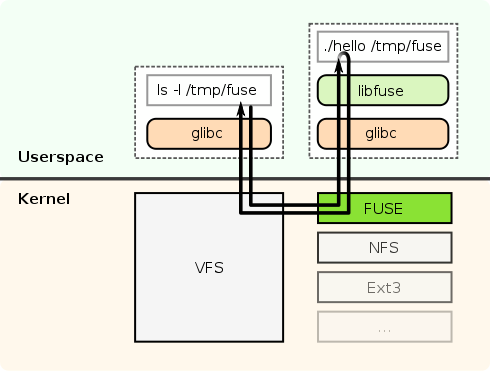
\includegraphics[scale=0.5]{./fuse.png}
\caption{Il flusso generato da FUSE}
\label{fig:1}
\end{figure}

Non tutte le funzioni, infatti sono richieste per avere un filesystem funzionante: alcune di essere sono dedicate a dispositivi speciali, altre, invece, fanno parte di un set che offre funzionalità aggiuntive. Nel nostro progetto è stato deciso di implementare un set che permetta di eseguire tutti i comandi essenziali in Unix (ma non è questo il lavoro che sè ne occupa).

Inoltre, a partire dalla versione 2.4 di FUSE, è possibile aggiungere un qualsiasi filesystem realizzato dal file \emph{fstab}.

\section{Perchè FUSE?}
Come abbiamo visto, sembra evidente che Fuse aggiunga un sufficiente \emph{overhead} rispetto all'uso di un filesystem come potrebbe essere Ext4 o Ext3, quindi, perchè scegliere FUSE?

La risposta più generica che si può dare è che è un metafilesystem versatile, potrebbe essere utilizzato per effettuare delle prove, ma non esiste \emph{il} perchè usare FUSE. Ciascuna implementazione di un filesystem ha delle proprie pecularità, e quindi ciascun utente potrebbe avere delle necessità per cui usare questo sistema.

Un esempio è costituito da WebDrive, un filesystem con cui è possibile utilizzare in maniera trasparente il servizio Amazon S3, o GmailFS, con cui è possibile memorizzare dati utilizzando lo spazio messo a disposizione da Gmail.

Il lavoro che abbiamo deciso di realizzare offre un servizio complesso e, si spera, utile. Utilizzando un database non relazionale potente come OrientDB in accoppiata alle API Blueprints, si intende fornire un servizio di memorizzazione che sia effettivamente fruibile a tutto tondo.

Innanzi tutto il progetto prevede la distinzione di un processo client e di uno server: il filesystem è implementato nel primo. Quando questo riceve una richiesta, verifica la possibilità di contattare il server; se questo è disponibile, gli viene chiesto di attuarla, utilizzando le API che verranno discusse nel capitolo successivo. Se tutto va a buon fine, il server notifica al client il risultato dell'operazione, che a sua volta restituirà i dati al processo che ha invocato la chiamata iniziale.

Una tale architettura permette, oltre che la semplice esecuzione del filesystem in un ambiente locale, la condivisione contemporanea degli stessi dati in remoto tra più utenti, mantenendo la politica dei permessi tipica di Unix.

Utilizzato in locale, invece, permette di condividere il filesystem tra più utenti proprio come si trattasse di una pendrive, con il vantaggio aggiuntivo che può essere spedito per mail, ad esempio, o caricato su un servizio di hosting.

Infine un altro motivo che ha fatto nascere questo progetto è stata la volontà di partecipare ad un progetto open source rispondendo alle richieste del gruppo di OrientDB.

